\documentclass[letterpaper]{article}

\usepackage{natbib,alifeconf,amsmath}  %% The order is important


% *****************
%  Requirements:
% *****************
%
% - All pages sized consistently at 8.5 x 11 inches (US letter size).
% - PDF length <= 8 pages for full papers, <=2 pages for extended
%    abstracts (not including citations).
% - Abstract length <= 250 words.
% - No visible crop marks.
% - Images at no greater than 300 dpi, scaled at 100%.
% - Embedded open type fonts only.
% - All layers flattened.
% - No attachments.
% - All desired links active in the files.

% Note that the PDF file must not exceed 5 MB if it is to be indexed
% by Google Scholar. Additional information about Google Scholar
% can be found here:
% http://www.google.com/intl/en/scholar/inclusion.html.


% If your system does not generate letter format documents by default,
% you can use the following workflow:
% latex example
% bibtex example
% latex example ; latex example
% dvips -o example.ps -t letterSize example.dvi
% ps2pdf example.ps example.pdf


% For pdflatex users:
% The alifeconf style file loads the "graphicx" package, and
% this may lead some users of pdflatex to experience problems.
% These can be fixed by editing the alifeconf.sty file to specify:
% \usepackage[pdftex]{graphicx}
%   instead of
% \usepackage{graphicx}.
% The PDF output generated by pdflatex should match the required
% specifications and obviously the dvips and ps2pdf steps become
% unnecessary.


% Note:  Some laser printers have a serious problem printing TeX
% output. The use of ps type I fonts should avoid this problem.


\title{ALIFE2022 template}



\title{Inferring Dynamic Parameter Relations from Experimental Probability Distributions}
\author{Anonymous Author$^{1}$, Anonymous Author2$^{1,2}$ \\
\mbox{}\\
$^1$California Institute of Technology, Pasadena, CA 91125 \\
$^2$California State University, Northridge, CA 91330 \\
anon@ymous.com} % email of corresponding author


% For several authors from the same institution use the same number to
% refer to one address.
%
% If the names do not fit well on one line use
%         Author 1, Author 2 ... \\ {\Large\bf Author n} ...\\ ...
%
% If the title and author information do not fit in the area
% allocated, place \setlength\titlebox{<new height>} after the
% \documentclass line where <new height> is 2.25in



\begin{document}
\maketitle

\begin{abstract}
% Abstract length should not exceed 250 words
    We present a novel method for relating experimental probability
    distributions of multistable systems to the parameters of a
    multistable model. We demonstrate that when such probability 
    distributions are fixed this implies that there is a fixed
    set of relations among the model parameters. Such relations 
    can help make predictions of parameters that aren't measured
    from ones that are. We apply this method
    to the canonical example of a bistable dynamical system: the cubic
    system.
    As well as to two theoretical models one of planerian regeneration
    and one of infant prehension learning.
\end{abstract}

\section{Introduction}
Biological systems are characterized by their robust stability under
a wide range of conditions. This is in part achieved by the ability
of such systems to take on different stable states
depending on contextual factors. One set of mechanisms that allows for such 
behavior is the presence of multiple long term stable states. Multistability
appears in a vast range of biological process ranging from microscale
genetic networks to macroscale population interactions. Across many levels 
of time and space biological systems seem to be able to adapt to new contexts
by maintaining multiple dominant stable modes.

Multistability has also
emerged as a useful tool in a explaining a large range of experimental phenomena.
Unlike theoretical models however, in the experimental context stochasticity
is unavoidable. As a result a common empirical practice is to sample what 
would be in the model, many possible trajectories of the system until they
reach equilibrium. 
Such sampling leads to a distribution of the stable states expressed as 
probabilities. This allows the experimenter to characterize the attractor
landscape and identify the range of possible equilibria.

Developmental dynamics are a particularly interesting case of multistability. 
Developing systems whether behavioral or morphological demonstrate multistability 
that is not only context decedent but expresses deep regularity in the timing of 
state transitions. In the case of behavior this can be observed in the existence
of critical periods or the milestones like progression developmental stages. 
In the case of morphological development we see this in the stage structure of
embryogenesis. A mechanistic understanding of how such regularity emerges is 
still in it's infancy.

In the context of the probabilistic approach used to experimentally 
study multistability, this regularity manifests as an observable oddity.
The probability distributions of developing systems ending up in a given
state is uncharacteristically consistent across different individuals 
in what would seem to be different conditions. The intuitive assumption
would be that each system would show a unique probability distribution
dependent upon individual factors. Instead, we observe that the probability
distributions are consistently species specific rather than individual specific.

Two examples of this phenomenon are the regeneration of the planerian flatworm
and the learning of reach-to-grasp in infants. In the case of planerian
theoretical models reveal how under certain environmental conditions 
planerian can develop into two possible configurations. In a natural context
the planerian when cut in two will regrow. The tail will regrow a head and the
head will grow a tail. However, experimental data from the Levin lab shows that
if the local electrical potential in the environment changes it is possible for 
a worm head to grow another head. Even, stranger is that if the potential
is altered only slightly, cryptic worms will emerge. Cryptic worms when cut 
may grow another head or a tail. In the case of the tail the child worm is 
also cryptic, even if returned to a normally polarized environment. The oddity
is that as long as the worm is cryptic the head-tail growth probability is $70\%$
regardless of the degree of polarization. This fixed probability is unexpected 
based on the basic theoretical assumptions one would make based on models of the
system.

Similarly, infant
prehension can be modeled as bistable: reach without grasp as one state
and reach with grasp as another, the system expresses both possibilities in the right
environmental context. Although an unexpected experimental finding is that in
both cases: the probability distributions across surprisingly large changes
to the relevant context remains relatively static. Infants maintain an extended 
period in which grasping starts to occur at a fixed probability. This is not a gradual
increase but rather a phase transition where for an extended period of time the probabilty
of reaching with and without grasping stays the same.
From a theoretical standpoint this seems 
counter-intuitive since changes over time and across infants would be expected 
to shift the basins of attraction and hence change the resultant probability 
distribution. Instead we see a period of relatively static probability.

Although, the source of this phenomena may be system specific and rely on deep
biological principles it serves as a fascinating example where the theoretical 
tools of dynamical systems could serve as a means of making experimental predictions.
In this work we propose a method to exploit such multistable regularity. We consider
theoretical models for both of these phenomena and identify how fixed 
probabilities provide a set of constraints on the relationship between model
parameters. This allows us to make predictions as to what various parameter 
values should be. We start by demonstrating the method in a simplified model
of bistability  then extend it to models of both flatworm regeneration and
prehension development.

\section{Results}
In the following sections we first introduce our method by motivating
and applying it to a toy model which is a popular mathematical model
of bistability. Once we work through the method in this simplified 
context, we apply the same technique to the two mentioned systms and 
identify where approximations or assumptions need to be made.

\section{The Cubic Equation}
To make the method clearer we imagine a hypothetical developmental
process. An alien is born yellow. As the alien ages depending
on various factors it may turn cyan or magenta. After much experimental observation
and some intense curve fitting, we identify a model that predicts 
which color a member of this alien species will become. The model is a dynamic
model that assumes that the color is a one dimensional variable that reaches 
an equillibrium at either cyan or magenta. In this case our hypothetical developmental
process is modeled as a cubic equation.

\begin{eqnarray}
    \dot{y} = \beta_1 + \beta_2 y + y^3
\end{eqnarray}

In this case $y$ represents the color of the alien. $\beta_1$ and $\beta_2$ are model 
parameters that vary across different alien clusters. In this equation $\beta_1$ and
$\beta_2$ are linearly separable so it is easy to distinguish their contributions 
to the model. $\beta_1$ specifies the x-intercept of the vector field function,
thus determining the exact position of the equillibria and $\beta_2$ dictates the 
curvature of the function. We visualize these contributions in Figure \ref{fig1}. 
Having sufficient curvature as well as an x-intercept
within the curvy region are both necessary for the model to display bistability.
In the language of development we may think of $\beta_1$ as the instructive parameter 
that says what the
specific outcomes will be and $\beta_2$ as the permissive parameter that defines the
range of possible outcomes.

\begin{figure}[t]
\begin{center}
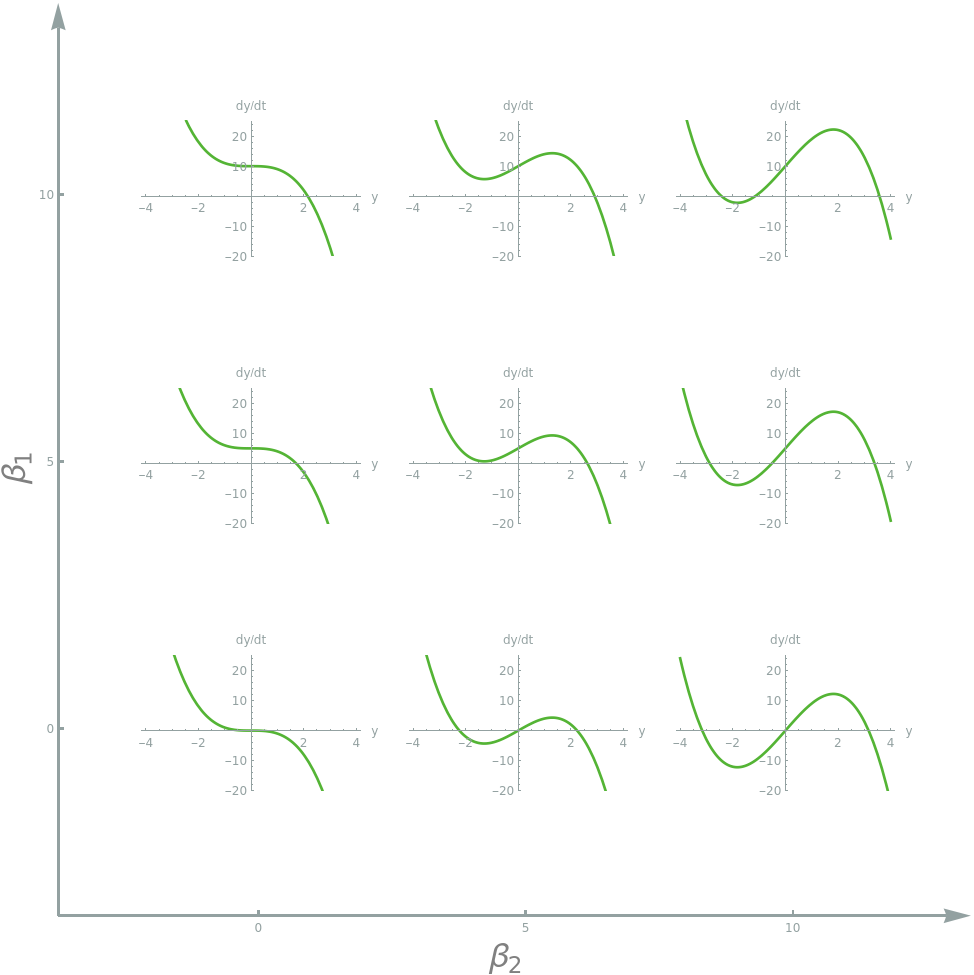
\includegraphics[width=2.1in,angle=0]{./cubic_params.png}
\caption{The effect is that $\beta_2$ determines the curvature around the 
center (horizontal)
and $\beta_1$ determines where the function reaches equilibrium (vertical).
If x-intercept is within the curved region this is an example of bistability.}
\label{fig1}
\end{center}
\end{figure}

We choose the cubic equation for our alien example because it is one of the 
simplest representations of a multistable system. It is a 
two parameter system where the appropriate range of parameters exhibits bistable
dynamics. Any initial condition will end up in one of two stable states. In this
case these states are the magenta or cyan skin color.

The aliens are very protective of their young and the experimenters are not able
to observe the process of many aliens coloring to maturity. However,
it is possible for an experimenter to join a cluster of adults and count
how many of each color there are. This is a common case in many experimental 
situations since it is often
easier to sample developmental outcomes than it is to sample longitudinal developmental
trajectories. Luckily our dynamical model gives us an intuitive way of thinking about
what those counts mean. If we imagine each individual as a specific trajectory through
the state space of the model then we are simply sampling initial conditions and counting
how many end up in each basin of attraction, we visualize this in Figure \ref{fig2}. Each
colored point represents an individual and the color represents their color after
the developmental process. Notice that the red saddlepoint acts as a divider. Points to
the left are cyan and to the right are magenta. This is because attractor basins in a 
dynamical system are seperated by an unstable manifold which is a poin in the 1D system.
The structuring of the state space by the saddlepoint allows us to constrain our model.

\begin{figure}[t]
\begin{center}
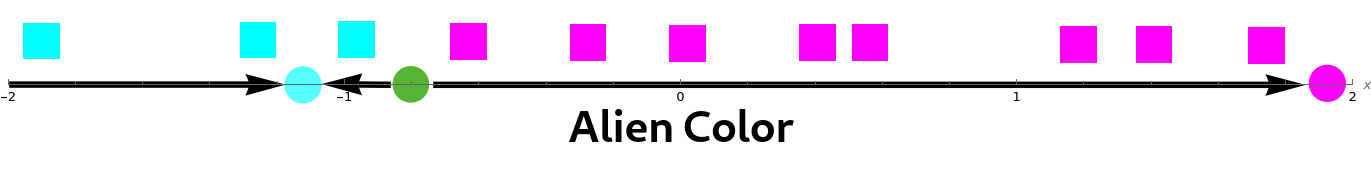
\includegraphics[width=2.1in,angle=0]{./basins.png}
\caption{Here we see the phase portrait of the system. The blue points represent
the stable equillibria and the red point is the saddle node. The magenta volume
represents the region of points that will end up in one basin and the cyan volume
represents the rest of the volume which will end up in the other basin of attraction.
The points above the volumes represent sampled trajectories colored by the basin they will
end up in.}
\label{fig2}
\end{center}
\end{figure}

Interpreting each point as a sampled trajectory, we would expect that by 
counting more individuals we would
get a good sense of the relative size of the two basins of attraction. Our model
predicts that the relative size of the basins of attraction is a function of the saddle
point location. We can even solve for the saddle
point using tools from dynamical systems theory. The saddle point ($SP$) is a point where the
vector fiel equation equals 0 and the derivative of that equation is positive (cite).
Solving for those criterion we get:

\begin{eqnarray}
SP = \frac{\sqrt[3]{-6} 
\left(\sqrt{81 \beta_1^2-12 \beta_2^3}-9 \beta_1\right)^{2/3}-2 
(-3)^{2/3} \beta_2}{3\ 2^{2/3} \sqrt[3]
{\sqrt{81 \beta_1^2-12 \beta_2^3}-9 \beta_1}}\\
    SP = f(\beta_1,\beta_2)
\end{eqnarray}

Although a little hairy, we were able to derive this function analytically.
This equation tells us that the saddle point position is a 
function of the variables $\beta_1$ and $\beta_2$. 
Depending only on these parameters we
can determine where the saddle point will be. These parameters therefore also determine
the sizes of the basins. Since we are interested in a generalized method we will abstract 
away the specific function and instead define $f(\beta_1,\beta_2)$.
$f$ is thus a function of the parameters that gives the value of $x$ at which the
saddle point lies. Such an $f$ will exist
in all two parameter 1D systems, however may require numerical approximations rather than
the analytic approach we took in this case. In the most general case the only 
requirement is that $f$ takes only
model parameters and returns the saddlepoint location.

The alienologists find a fascinating result that there
are always 3 cyan aliens for 7 magenta aliens. This seems to be the case regardless
of which cluster they observe. This is odd because many alienologists have
also observed that the parameters can vary in different clusters. Meaning that we see 
different $\beta_1$ and $\beta_2$ values across different clusters.
If we consider this puzzle in the context of our dynamical
model, one way to interpret is that we observe a fixed ratio of the basins of
attraction. Intuitively this shouldn't be the case since the different
clusters have different parameters which would imply different basin boundaries. Although
seemingly contrived, as will be detailed later, this situation seems to occur in the two
example development systems we will discuss in the next sections.

The method we propose assumes that both the interpretation of the model and the experimental
observations are correct. Given these conditions we demonstrate 
how we can make experimental predictions about the relationship between the 
parameters $\beta_1$ and $\beta_2$.

First we must make some assumptions
about how the experiment is conducted. Specifically we need to define a sampling
distribution $P(x)$. $P(x)$ is a probability density function that 
tells us how likely a state interval $a<x<b$ was to be sampled during the experiment. 
To sensibly discuss the ratio of basin boundaries we need finite volumes for each basin.
This must also be accounted for in $P(x)$. This can be done by either selecting a $P(x)$
with a bounded cumulative distribution function like a normal distribution or by selecting
a sampled state interval. For this paper we will take the latter approach but in a real
experimental system, the former might be more appropriate. To justify our boundaries
we start with the observation that not all possible states are likely to be sampled.
There will be values of $x$ that are never actually observed, which should have probability 
0. In our alien context we
do not expect baby aliens to be born of every possible color. 

For theoretical simplicity
we will assume this sampling bias takes the form of an upper and lower limit. 
This means that all $x$
below some $x_{min}$ and all $x$ above some $x_{max}$ will have a probability of 0. 
We will also assume that within these bounds that the experimenter
may observe any possible trajectory with equal probability. These combined assumptions 
equate to imagining that experimental sampling is uniform across a region of the state 
space. We consider a uniform $P(x)$ since this is also the maximum entropy distrubition.
Once again in an experimental context the method can be improved
by using known sampling distributions based on experimental observation. Mathematically,
the only restriction is that we assume the integral is bounded. 

\begin{eqnarray}
    P(x) = \begin{cases}
        \frac{1}{x_{max} - x_{min}} & \text{ for } x_{min}\leq x\leq x_{max}\\
        0 & \text{otherwise}
    \end{cases}
\end{eqnarray}

Given we have a sampling distribution $P(x)$, we can use our knowledge of the dynamics
to determine the probability of sampling a cyan or magenta alien. Since we are dealing
with a 1D system whether a given $x$ will end up in the cyan or magenta basin of attraction
is determined by whether $x$ is greater or equal to the $SP$. If $x$ is less than
$SP$ it will end up in the cyan basin of attraction otherwise it will
end up in the magenta basin of attraction. We can calculate the probability of $x$ ending
up in the cyan basin by integrating the probability of sampling $x$ 
from the minimum observed $x_min$ up to $f(\beta_1,\beta_2)$.

\begin{eqnarray}
    P_{cyan}(x) = 1 - P_{magenta}(x) = \int^{f(\beta_1,\beta_2)}_{x_{min}}
    P(x) dx
\end{eqnarray}

Intuitively this is the cyan volume in Figure \ref{fig1} divided by the total volume
of cyan and magenta. 
Once again we see that this only depends on the parameters $\beta_1$ and
$\beta_2$. This means that by varying $\beta_1$ and $\beta_2$ we can get different 
probability values. Every pair of parameters $\beta_1$ and $\beta_2$ will define a 
value for $P_{cyan}(x)$.
We can plot this probability as a 2D surface in a 3D space, where the axes
are $\beta_1,\beta_2,P_{cyan}(x)$ (Figure \ref{fig3}). For $\beta_1$ and $\beta_2$ where
the system is not bistable this will be either 1 or 0, which we can ignore. For the bistable
ragion we get a continious 2d manifold. As expected the manifold should resemble the 
parameter chart of the system but embedded in a higher dimensional space.

We can gather some intuition about the expected probabilities just by looking at the 
surface. We notice that the surface
does not extend to all parameter values. This is because there is a range of possible
parameterizations for the cubic where bistability persists. In our cubic this could
be either because the function does not exhibit sufficient curvature to permit bistability 
or because the x-intercept is above or below the appropriate region.
The orientation of the surface relative to the probability axis tells us how sensitive the 
probability is to parameter choice. The fact that the manifold is relatively flat along the
$P_{cyan}(x)$ dimension implies that the probability is not vert sensitive to parameter choice
in general. These properties are useful for experimental evaluation of a dynamical model
more generally. They will also differ across the different models in this paper.

\begin{figure}[t]
\begin{center}
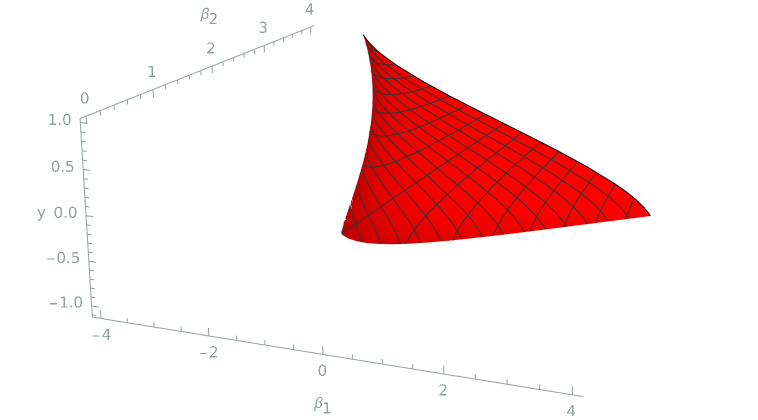
\includegraphics[width=2.1in,angle=0]{./saddle_cubic.png}
\caption{This is the surface of the saddle point location as a function of
the parameter $\beta_1$ and $\beta_2$. The manifold is embedded into probability
dimension representing the probability of a trajectory leading to the cyan attractor.}
\label{fig3}
\end{center}
\end{figure}

Now that we have visualized the necessary theoretical construct we can make use of  
the experimental data. In the case of the aliens, we observed a 
fixed probability distribution of alien colors. 
Specifically we said that, we always observe a $30\%$ chance of finding cyan aliens. 
In the case of our plot this is equivalent to drawing a plane in the 3D space that 
intersects the probability axis at $0.3$. We can see this in Figure \ref{fig4}. Point
that lie on the intersection between this plane and the manifold are points in parameter
space where bistability exists and $P_{cyan}(x)$ matches the experimentally observed 
probability distribution. In this case the intersection defines a line. Since our observed
probability is a constant we only consider a plane intersecting the manifold which would
define either one or several such lines. In the more complex case of a volume of probability,
for example if we observed a distribution with variance, we would see a more complex 
structure. We can solve for the exact value of this line by considering $P_{cyan}(x) = 0.3$.

\begin{figure}[t]
\begin{center}
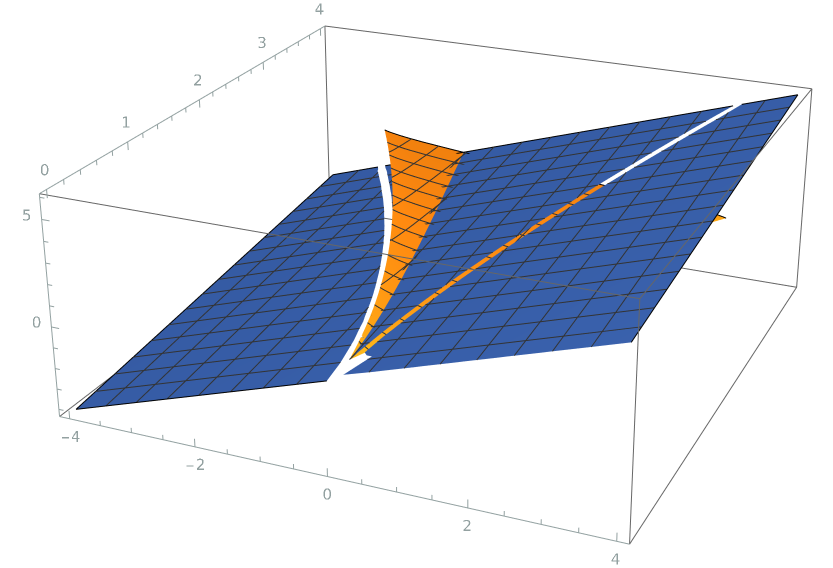
\includegraphics[width=2.1in,angle=0]{./cubic_pg.png}
\caption{This is the surface of the saddle point location as a function of
the parameter $\beta_1$ and $\beta_2$.}
\label{fig4}
\end{center}
\end{figure}

\begin{eqnarray}
    P_{cyan}(x) = 0.3 = \int^{f(\beta_1,\beta_2)}_{x_{min}}\\
    \beta_1 = 0.343 - 0.7\beta_2
\end{eqnarray}

Once again the simplicity of our example makes it possible to analytically solve this problem
by taking the inverse of the integral, in general however, we might need to make a numerical
approximation to be able to determine this relation. This will come up in the later examples.
This line is a fixed relationship between
the two parameters, $\beta_1$ and $\beta_2$ that must be satisfied for us to 
unify the experimental observation with
our model. Hence we expect that if the experimenters were to measure $\beta_1$ and 
$\beta_2$ they would fall on the line satisfying the equation. An alienologist 
should then be able to predict $\beta_1$ or $\beta_2$ given that they
know the other. This relation thus gives us a whole new way to validate or
falsify our original model. 

Now that we have established the steps to apply the method in a simple case we will now 
consider the same sequence of operations in the case of two models of real world experimental
systems. Although we may need to use numerical approximations and our parameters may not
be easily interpretable we will see that the same steps can be applied.

\subsection{Infant Prehension}

Infant prehension or reach-to-grasp is an important developmental milestones 
for many primates including humans (cite). Not only is the behavior itself
functionally important (cite) but also serves as a foundation for more general motor
coordination skills (cite) and many social skills (cite). The development of reach-to-grasp
has therefore been an important model system in the study of human development (cite). 
One way of modeling prehension development has been to look at a phase transition
between reach and reach-to-grasp. Infants begin to reach before they preform grasps and
one set of hypothesese has interpreted this as a phase transition into bistability (cite). 
Experimental work in this direction has been complemented by modeling of this phase
transition. This makes prehension a potential model system for exploring developmental
dynamics with the tools of dynamical systems theory.

Much like our alien example, experiments in prehension development have shown that after
the emergence of grasping we observe a narrow probability distribution while bistability
remains. Although infants eventually will grasp with every reach until then there seems to
be a fixed probability distribution of reaching-to-grasp and reaching-without-grasp (cite).
We will treat this as meaning there is a constant probability across both stable outcomes,
however, extensions of this work could extend the method to more complex distributions.
Either way the fact that the probability distribution is narrow is still enough to suggest
there may be an important relation between the model parameters.

There is a major different between this example and our previous example however. 
In the previous  section we demonstrated how this method can be applied to a simple
toy model and how given an experimentally observed probability we could make a prediction
about the model parameters. In many cases the exact model parameters are 
not singular observables but instead are a function of observables. In such cases we 
must accommodate the method by relating the saddle point position not to the model
parameters but to the desired experimental observable.
This will be the case as we apply the method to a model of the development of 
reach-to-grasp in infants. 

We consider the dynamical model of prehension development proposed by Wimmers (cite). This
model considers two stable states: reach-to-grasp and reach-without-grasp. To develop this
model the researchers looked at many possible parameters and considered their effect on 
the resulting probability of either of the bistable outcomes. They found that the results
were best explained a by version of the cubic equation.

\begin{eqnarray}
  \beta_1 + \beta_2 (\frac{x-51.04}{26.98}) - (\frac{x-51.04}{26.98})^3
\end{eqnarray}
where
\begin{eqnarray}
  \beta_1 = 5.98 - 1.07c + 31.92w\\
  \beta_2 = 5.56 - 0.25c + 0.38w
\end{eqnarray}

Notice that this equation is quite similar to the cubic however both $\beta_1$ and 
$\beta_2$ are linear sums of other parameters: $c,w$ where $c$ is the arm circumference
of the infant and $w$ is the arm weight. The value of $x$ is shifted linearly this does 
not affect the actual dynamics and is ignored for methodological clarity. We are no longer
interested in how the values of $\beta_1$ and $\beta_2$ relate to $SP$. Instead we will
consider how $SP$ is related to $c,w$. However, almost all of the other steps will be the
same as in the previous example.

First we visualize the contributions of the paramaters to the dynamics (Figure \ref{fig5}).
Since the paramaters affect both $\beta_1$ and $\beta_2$ we cannot simply attribute 
curvature to one and x-intercept location to the other. Instead we see that both parameters
affect both of these properties however the contribution of $w$ to the x-intercept location
is significantly greater than the contribution of $c$. This will play a role in how the
manifold looks once it is embedded in the probability space (Figure \ref{fig6}).

\begin{figure}[t]
\begin{center}
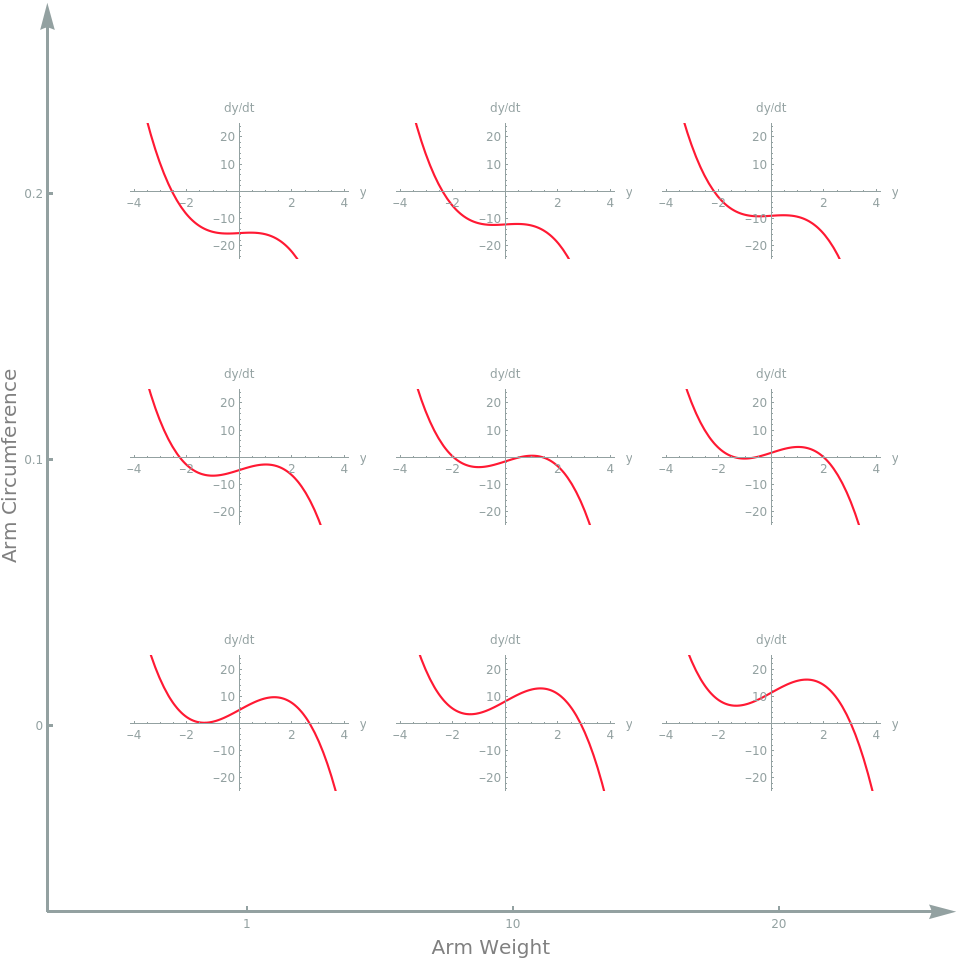
\includegraphics[width=2.1in,angle=0]{./prehension_params.png}
\caption{3x3 grid of variation in $c$(horizontal) $w$(vertical). Unlike the previous
model curvature and x-intercept position changes as a function of both parameters.}
\label{fig5}
\end{center}
\end{figure}

Once again we need to start by defining the relationship between $SP$ and the parameters.
This will again take the form of a function $f(c,w)$ that returns the saddlepoint location 
$SP$.
Luckily since $\beta_1$ and $\beta_2$ are only linear combinations of $c,w$ we can still
find the function $f(c,w)$ analytically. Once again we solve based on the previous conditions
and get the closed form function.

\begin{eqnarray}
  f(c,w) = placeholder
\end{eqnarray}

As before we select one outcome in this case reaching-to-grasp,
and find the probability that a sampled point will end up in the basin of
attraction of reaching-to-grasp rather than reaching-without-grasp. To do so we again
need to define a sampling distrubition. We again will do this using a bounded uniform
pdf for $P(x)$ which is identical to $P(x)$ in equation 4. The only difference being 
that the volumes represent whether the behavior is preformed rather than the alien
color. Using the same reasoning we can define the desired $P_{grasp}(x)$, the probability
that in a sampled point the baby will grasp, by integrating the volume. In this case
the desired volume is on the right so we integrate from $SP$ to $x_max$.

\begin{eqnarray}
    P_{grasp}(x) = \int_{f(c,w)}^{x_{max}}P(x)dx\\
\end{eqnarray}

Thus for any pair of $c,w$ we get a single scalar probability that is the probability
of a sampled reach including a grasp. We can plot this surface in the 3D space of 
parameters and probabilities (Figure \ref{fig6}). Once again we see this forms a 
2D surface in a 3D space however unlike before the orientation of the surface seems much
less flat. This means that for a small change in parameters we may get a large change in
the resulting probability. Other than however we still see that the surface resembles the 
cusp bifurcation we would see in the parameter chart.

\begin{figure}[t]
\begin{center}
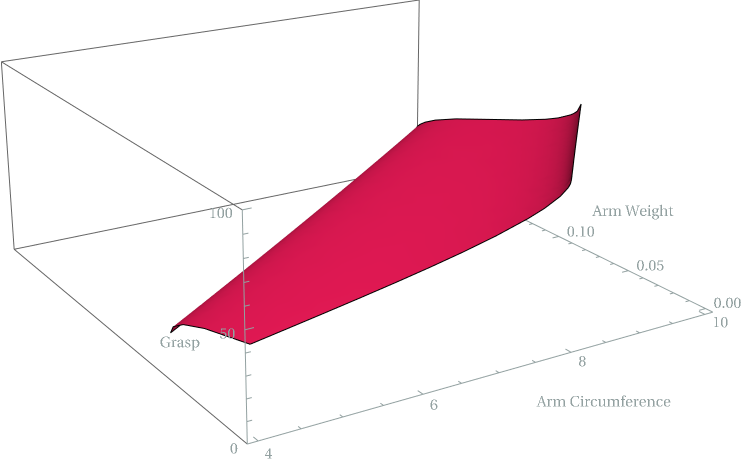
\includegraphics[width=2.1in,angle=0]{./saddle_prehension.png}
\caption{The probability we find as we vary saddlepoint by moving in the 
parameter space of $c,w$. The plane represents the observed constant probability 
distribution.}
\label{fig6}
\end{center}
\end{figure}

Since we are again considering the observed probability to be constant (0.5), we can once 
again draw a plane. As before instead of a plane we could draw a surface that is more complex
if we want to consider the observed probability as a distribution rather than a constant. The
plane is across all paramerer values $c,w$ and is centered at $P_{grasp}(x) = 0.5$
(Figure \ref{fig6}). Once again the intersection of the plane and the manifold will define
a line. This line can be solved for analytically again as before.

\begin{eqnarray}
  \text{prehension line}
\end{eqnarray}

This line, makes a prediction that the fixed probability distribution implies that the
relation between arm circumference and arm weight will
follow the equation 14. As one parameter varies the other should at a proportional degree.
We know have a prediction that can falsify or further validate the cusp model fit in the 
orignal paper (cite).

In this example we applied the same steps and method to a real world system. We showed how
more complex parameter relations can be accounted for by adjusting the function $f$ and how
different parameterizations might imply more complex relations to the resultant probabilites.
However, since our model was still cubic we were able to use much of the same analytical 
machinery. We will next consider a case where the model is much more complex, yet we will 
show with the use of numerical approximation how many of the same steps can be applied.

\subsection{Planerian Regeneration}

The final case we consider is a model of planerian flatworm regeneration. The dynamics 
of this system are much more complicated and many of the analyitcal tools we used
in the previous examples no longer apply. Instead, we will demonstrate how numerical
approximations may be used to fill in the gaps.

Planerian flatworm is a popular model system for several reasons (cite). Of particular
interest to us is it's regenerative capabilities. Work from the Levin lab (cite) has
provided a wide range of experimental results that has helped characterize the development
of this animal across many conditions. For this example we will consider axial patterning
in the flatworm.

Planerian can reproduce through an asexual cloning process. When a worm is cut into two
the head and the tail will both regrow the rest of the body. One interesting aspect of
this process is that it seems to be at least in part controlled by electrical signaling
rather than purely chemical signaling. This has been show through experimental manipulation
of the polarity of the environment during regeneration(cite).

Through manipulation of the polarity of the environment it becomes possible to cause
the planerians decapatated head to grow another head instead of a tail, resulting
in a two headed worm. Interestingly, there is a more surprising finding. It is also
possible to manipulate the polarity such that the worm regrows normally however if 
cut again the worm may grow another head or a tail stochasticlly. Such worms are 
called cryptic worms (cite). One unexpected experimental result is that near universally
cryptic worms have a $30\%$ chance of spawning into a two-headed worm and a $70\%$ chance 
of spawing another cryptic worm.

Many features of this phenomena have been successfully modeled using a bistable dynamical
model. Normal and double headed worms are modeled as living in parameter space without
bistability where as cryptic worms are thought to occuppy the bistable region (cite). 
This is the model we will use for the rest of this example.

\begin{eqnarray}
  \text{worm model equations}
\end{eqnarray}

We have simpliefied the model significantly from it's original formulation by replacing
parameters with their experimentally observed values. We have also reduced this from a 
2D to a 1D system by considering the difference in polarity between head and tail rather
than head and tail as seperate dimensions. This works in this case because the difference
in polarity is sufficient for applying the method.
This leaves us with two free parameters
$g_{pol},g_{max}$. $g_{pol}$ is the polarity of the gap junction between head and tail 
and $g_{max}$ is the maximum conductance across the gap junction.

Once again we will start by considering how the parameters affect the equillibria of
the model. This is will give us intuitions about how they may affect the probability
surface. We can visualize this in Figure \ref{fig7}. Although no longer cubic we 
see a similar pattern as before where one parameter mainly affects the curvature ($g_{max}$)
and one mainly affects the x-intercept location ($g_{pol}$). Although these parameters are 
definitely not linearly composable as before.

\begin{figure}[t]
\begin{center}
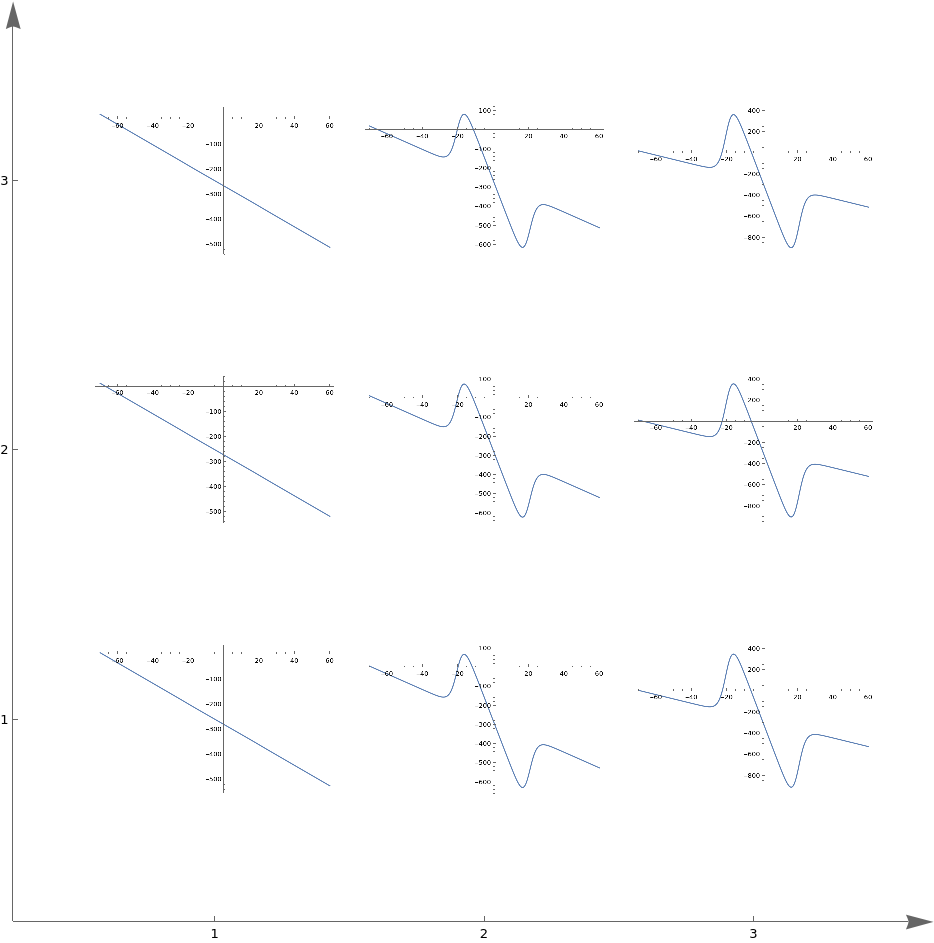
\includegraphics[width=2.1in,angle=0]{./worm_params.png}
\caption{Vector field function as we vary the two parameters}
\label{fig7}
\end{center}
\end{figure}

As before we go through the process of defining a function $f(g_{pol},g_{max})$ that
given the two parameters of the model will return the equillibria location. Unlike 
before we cannot simply solve for the conditions relevant to a saddlepoint. Instead
we must resort to numerical root finding. We identify an initial guess for the saddlepoint 
by looking at Figure \ref{fig7}. The middle intersection on the x-axis is the saddlepoint.
Using this guess we can generate a tensor whose first 2 dimensions are the parameters 
$g_{pol}$ and $g_{max}$ and whose 3rd dimension is the saddlepoint location. This also
defines a surface which we can plot (Figure \ref{worm_sp}).

\begin{figure}[t]
\begin{center}
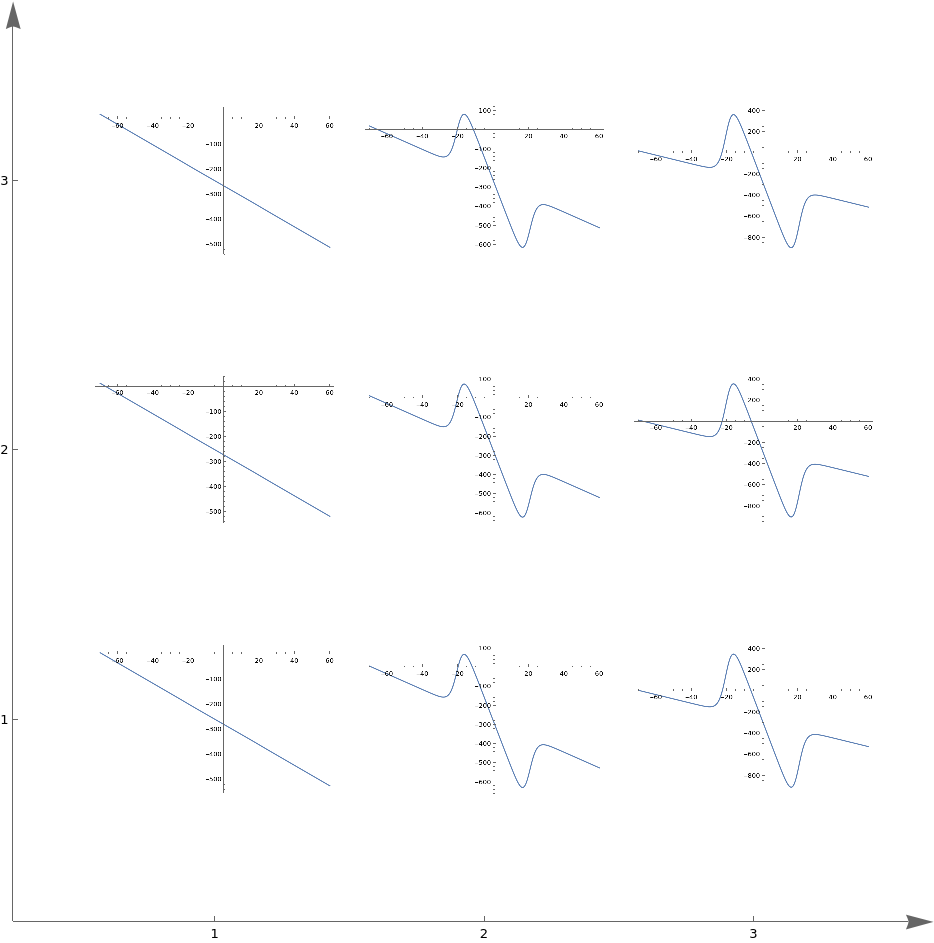
\includegraphics[width=2.1in,angle=0]{./worm_params.png}
\caption{Saddle point location as a function of the two parameters}
\label{worm_sp}
\end{center}
\end{figure}

Once again we want to convert from the saddlepoint position to a probability. Here we 
want the probability that a given worm will end up as two-headed. We define our sampling
distribution once again using a bounded uniform distribution $P(x)$ also identitical 
to equation 4. The two-head outcome is on the left side of the saddlepoint. Thus 
we know that finding $P_{two-head}(x)$ means integrating $P(x)$ from $x_{min}$ to
$f(g_{pol},g_{max})$.

\begin{eqnarray}
    P_{grasp}(x) = \int_{f(g_{pol},g_{max})}^{x_{max}}P(x)dx\\
\end{eqnarray}

Since $f(g_{pol},g_{max})$ is calculated numerically we must also numerically integrate the
function. Doing this across a range of parameters $g_{pol}$ and $g_{max}$ gives us another
2D surface which can be embedded in the 3D of the $P_{two-head}(x)$. Plotting this surface
we get Figure \ref{worm_prob}.

\begin{figure}[t]
\begin{center}
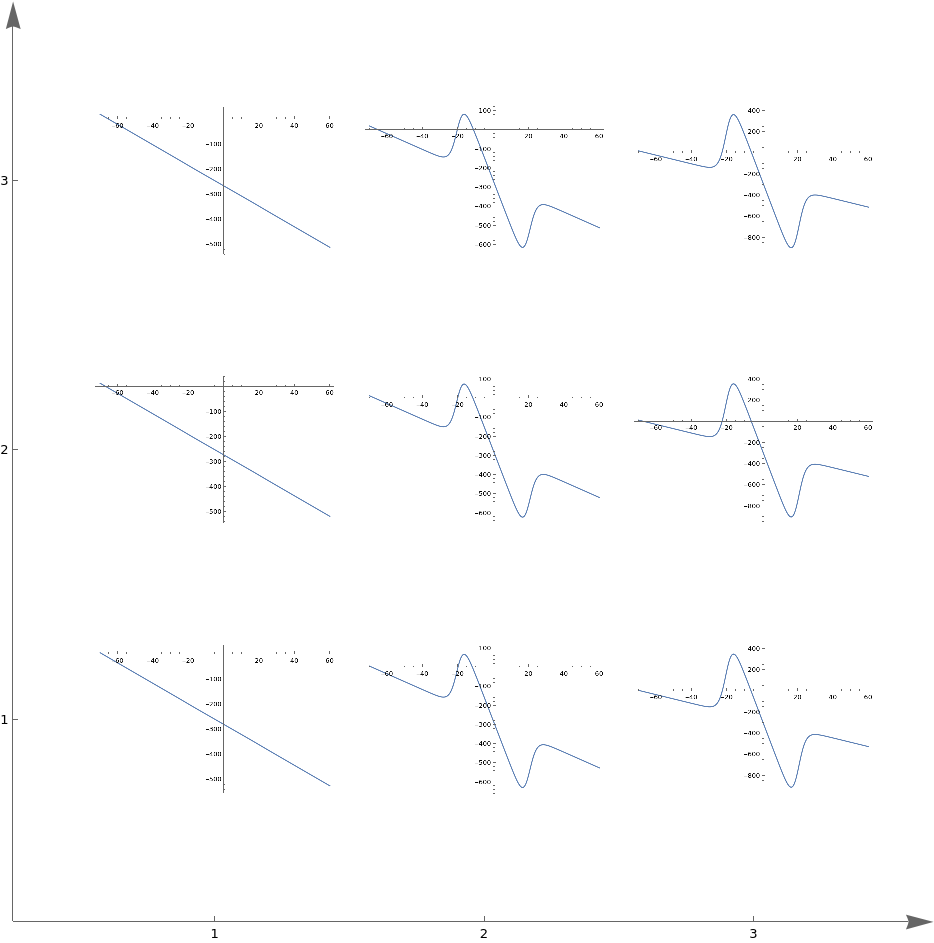
\includegraphics[width=2.1in,angle=0]{./worm_params.png}
\caption{Worm parameter manifold embedded in probability space}.
\label{worm_prob}
\end{center}
\end{figure}

The experimental evidence found a constant probability of spawning a second head to 
be $30\%$. We once again draw a plane through the manifold as before
(Figure \ref{worm_prob}). As before the plane and the manifold intersect along 
a line. However, the location of this line cannot be found analytically. Instead,
we solve for it numericaly and visualize it in Figure \ref{worm_line}.

\begin{figure}[t]
\begin{center}
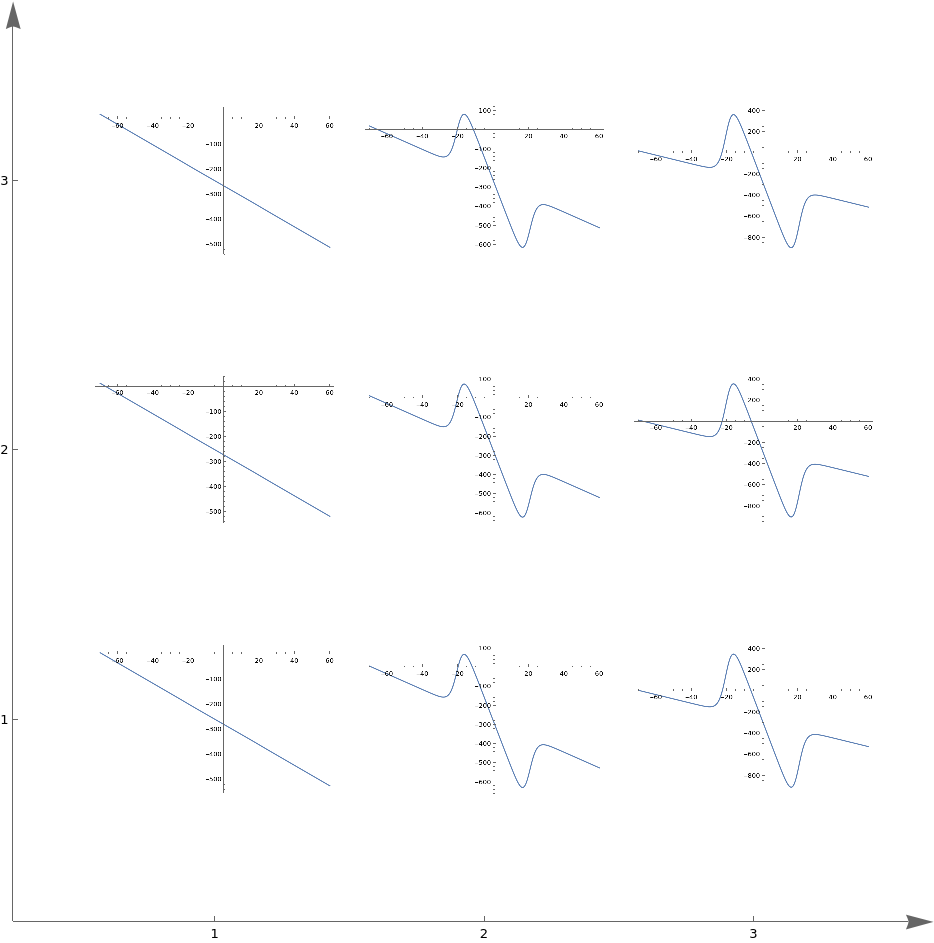
\includegraphics[width=2.1in,angle=0]{./worm_params.png}
\caption{Line relating $g_{pol}$ to $g_{max}$ that is bistable and meets the probability
criterion.}
\label{worm_line}
\end{center}
\end{figure}

Once again we can see how the constant probability distribution presents a set of 
constraints on the parameters of the dynamical model. In turn such constraints can
be used to make emprical predictions which can further validate or contradict the
model as a hypothesis. Thus we can make concrete predictions on what the parameters
should be even in the case of an extremely simplified theoretical model.

\section{Discussion}
In this paper we have demonstrated how our method can be applied to different
dynamical models to make concrete predictions about observable paramaters using 
a theoretical model in conjunction with experimental data. We also demonstrate
how this model can be applied to real world systems even when things become 
analytically intractable.

Although in this work we limited our model to a very simple sampling distribution,
using the known emprical sampling distrbution could greatly improve the accuracy of
the method without comprimising the conceptual steps, albeit with increased numerical
computationa time.

Future work may extend this method in many different directions. One example may 
be to introduce more complex parameter constraints than a constant probability
distribution. Having a range of possible probabilities will also reduce the
range of possible parameters for the models. Even more generally an observable
of the equillibria could be used with a similar method rather than simply
probabilities. As long as the function can be related to the equillibria of the
dynamics it can serve as a means of inferring necessary dynamical parameter relations.

Finally, we demonstrate that dynamical systems can not only serve as a set of conceptual
tools but also can help elucidate and imporove experimental results. There is much need
for growing communication between experiment and theory in biology and dynamical systems
can provide a firm foundation for such communication.
\section{Acknowledgements}

This work was supported by NSF grant No.\ PHY-9723972.

\footnotesize
\bibliographystyle{apalike}
\bibliography{example} % replace by the name of your .bib file


\end{document}
